\section{Two-Party Tests}
\label{sec:two-party}

Two-Party tests are the normal telephone calls between two participants.
User A calls another user (perhaps User B) who has to be registered, makes a phone call and hangs up.

As a \texttt{sip} dialog, the scenario looks as follows:
\begin{figure} [!ht]
\centering
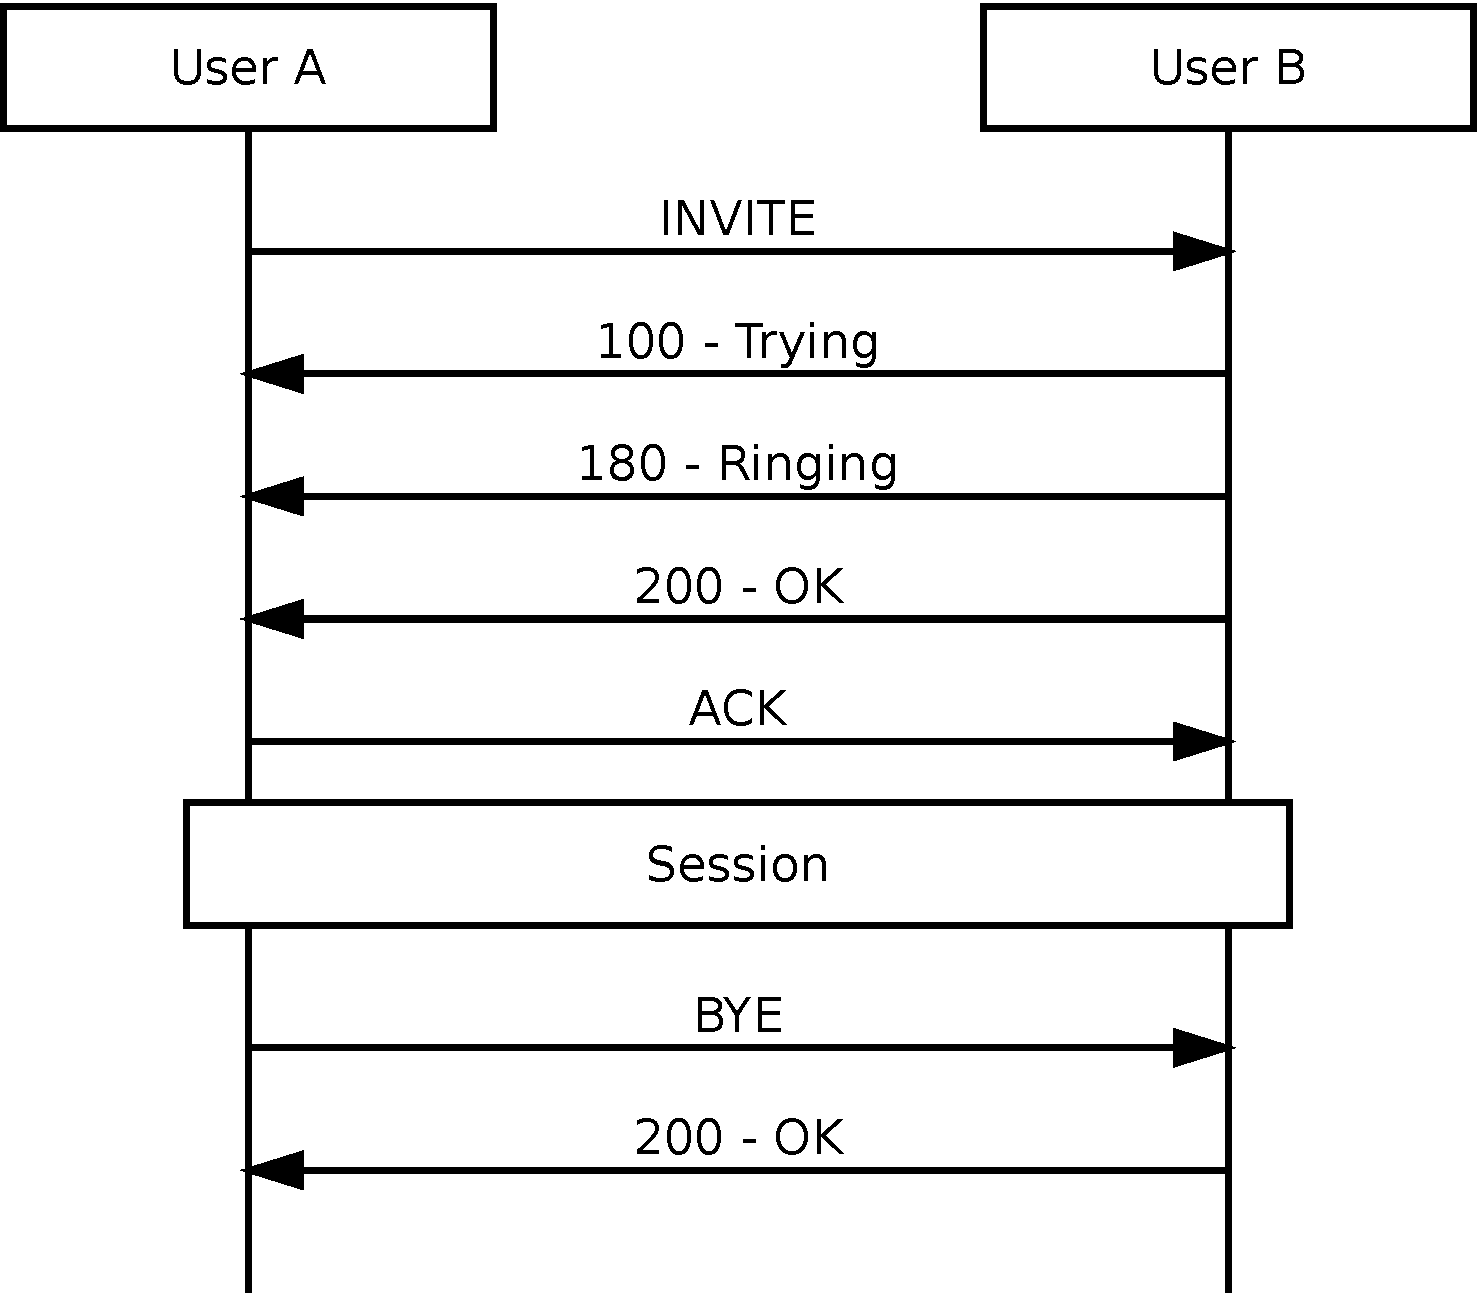
\includegraphics [width=10cm] {twoway-1}
\caption{SIP dialog of a two-party call}
\end{figure}
The original XML scenarios for sipp used to implement this are available in the appendix. \newpage

\begin{figure} [!ht]
\centering
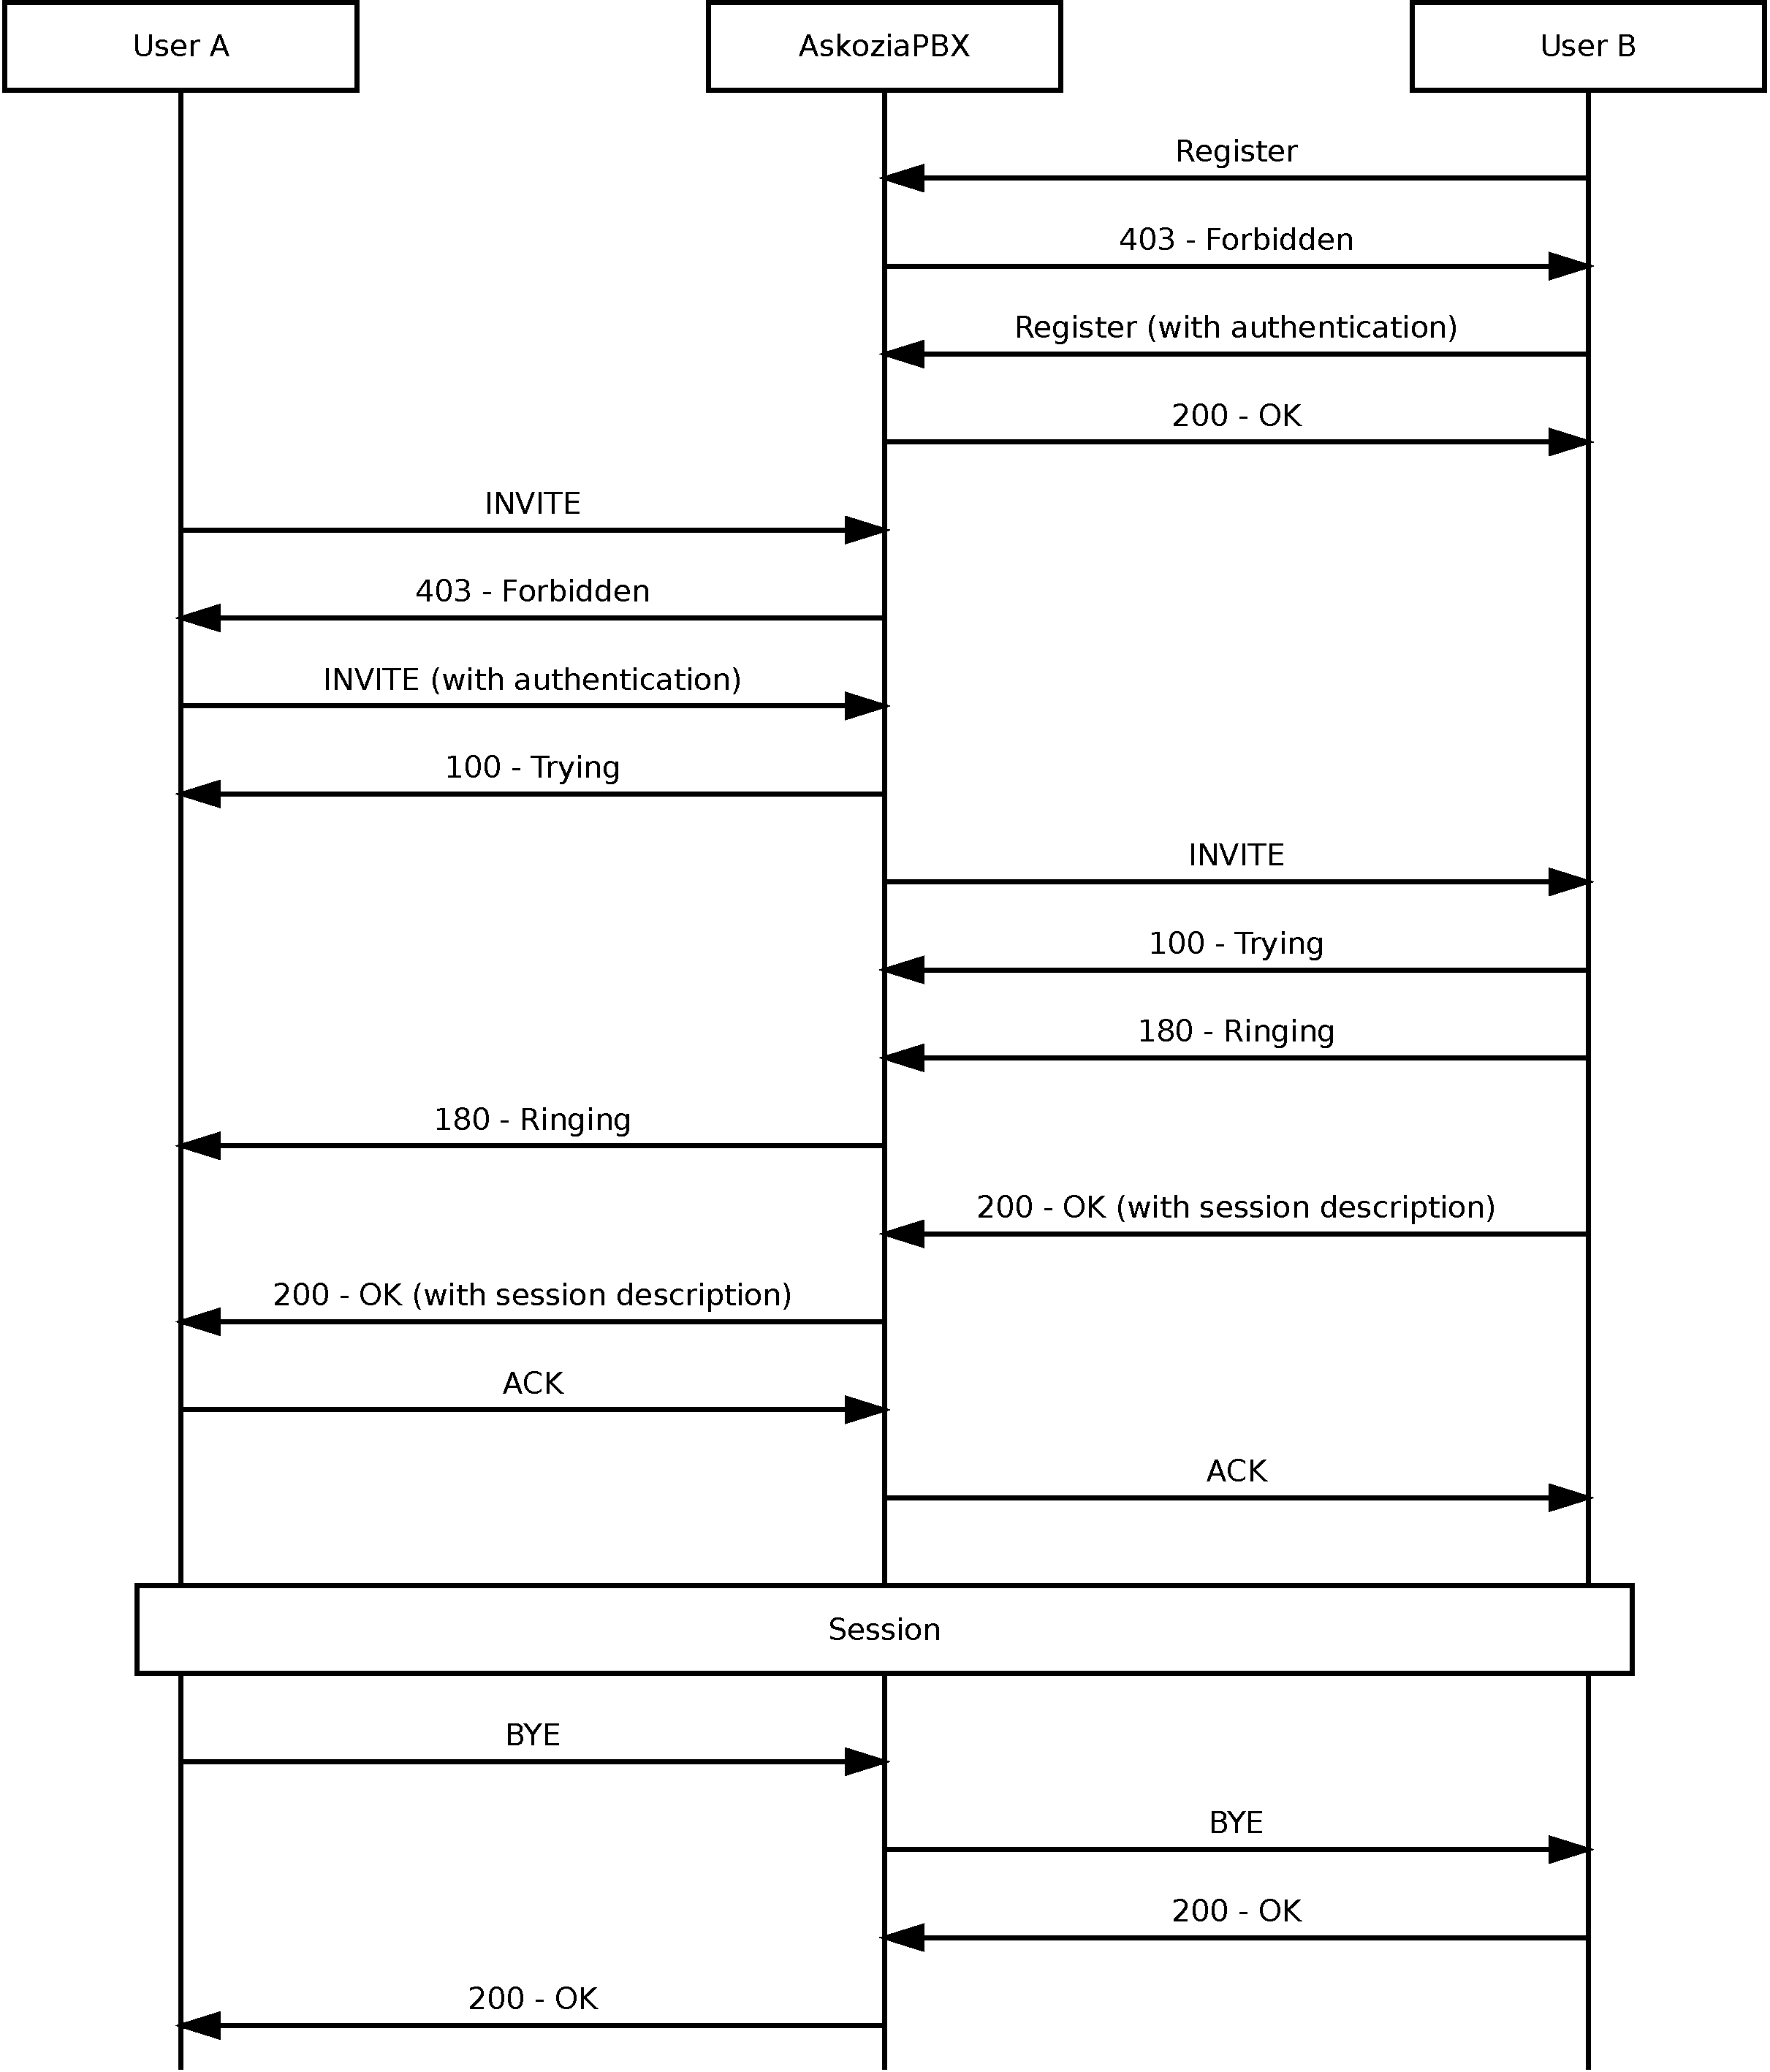
\includegraphics [width=15cm] {twoway-2}
\caption{Dialog of a two-party call}
\end{figure}

The next diagramm shows the process of a complete two-party test: \newpage
\begin{figure} [!ht]
\centering
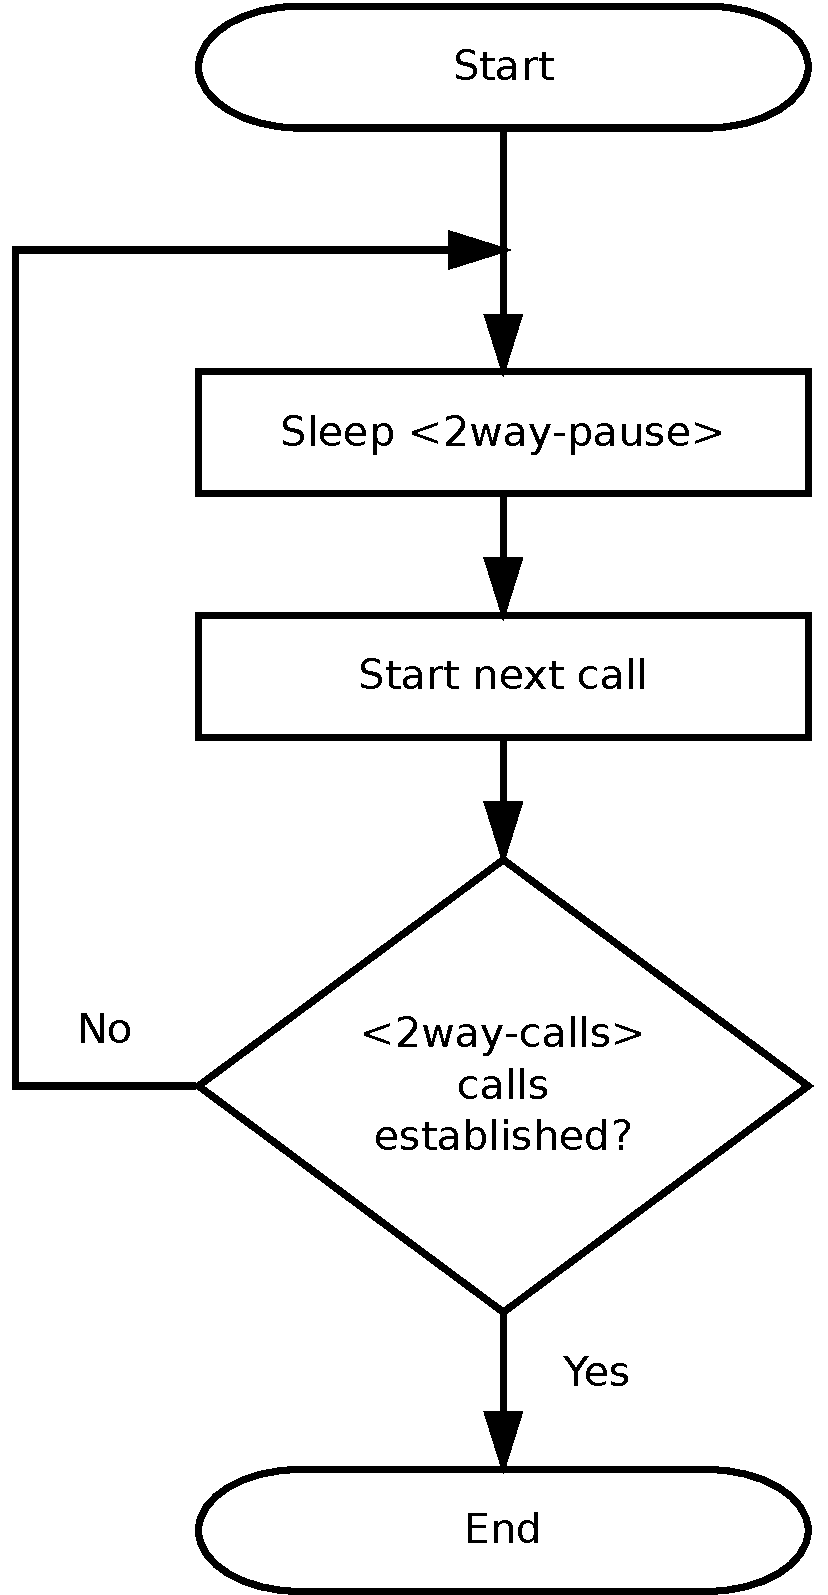
\includegraphics [width=6cm] {twoway-3}
\caption{Complete two-party test}
\end{figure}

The number of calls is increased step-by-step. After every call, the script waits for the specified pause
time to record the CPU load values. For executing two-party calls, the following sipp commands used.
You can inform yourself about the used parameters by reading the sipp manpage (the appendix contains the sipp manpage).
\begin{lstlisting}[breaklines=true,label=code:twoway-invite,caption={sipp command for inviting User B} ]
REGISTER Command:
$sipp -aa -inf '$users_twoway_file' -m $current_call -i $local_ip
  -p $sip_dst_port -mp $rtp_dst_port -sf '$reg_scen' $ask_ip 2>&1

ACCEPT Command:
sipp -aa -inf '$users_twoway_file' -m $current_call -i $local_ip
  -p $sip_dst_port -mp $rtp_dst_port -sf '$acc_scen' -bg $ask_ip 2>&1 &

INVITE Command:
sipp -aa -inf '$users_twoway_file' -m $current_call -i $local_ip
  -p $sip_src_port -mp $rtp_src_port -sf '$inv_scen' $ask_ip 2>&1

De-REGISTER Command:
sipp -aa -inf '$users_twoway_file' -m $current_call -i $local_ip
  -p $sip_dst_port -mp $rtp_dst_port -sf '$der_scen' $ask_ip 2>&1
\end{lstlisting}

